\section{Model testing}
Substituting all the constants of \eqref{2ndCubliTransferFunction} with the parameters of the real model results in the final transfer function of the system.
%
\begin{flalign}
	\eq{G(s)}{\frac{-133 \cdot s}{s^3 + 1,015 \cdot s^2 - 87,74 \cdot s - 2,487}} &\nonumber\\
	\label{RealCubliTransferFunction}	
\end{flalign}
%
Using \eqref{RealCubliTransferFunction} it is possible to simulate the response of the system to a step input and compare it with the response of the simulation of the block diagram. This is done to verify that the block diagram is in fact showing the system described in \eqref{RealCubliTransferFunction}, as seen in \figref{stepComparison}.

\begin{figure}[H] 
	\centering 
	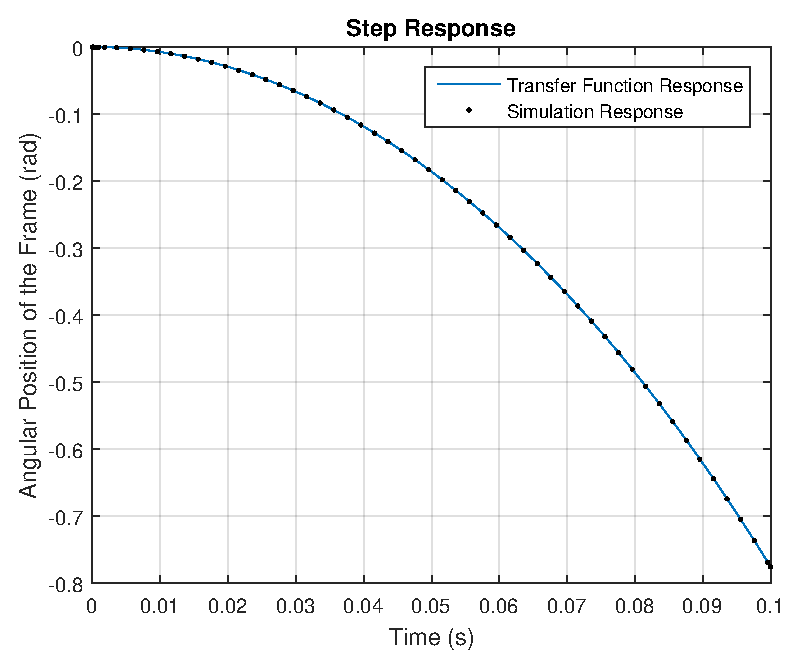
\includegraphics[scale=0.55]{figures/stepComparison}
	\caption{Step response comparison between the transfer function from \eqref{RealCubliTransferFunction} and the block diagram from \figref{cubliSimulink}. The conclusion form this is the blockdiagram of the system was made correctly}
	\label{stepComparison}
\end{figure}


In \figref{LinearizedVSNonlinear}, the effect of the linearization is apparent. In the simulation the frame is placed in upright position very slightly off \si{0\ rad}. The small deviation from \si{0\ rad} is applied in the last plant feedback, see \figref{cubliSimulink}. If, in the simulation, the model is started out at exactly \si{0\ rad}, it will balance in upright position.
\Figref{LinearizedVSNonlinear} shows the behavior around the frame's pivot point and does not include the platform itself. For this reason, the simulation allows for the frame to fall down and act as a normal pendulum. The nonlinear model shows how the pendulum dampens around its natural equilibrium point, while the linear model keeps increasing the angle.
However, in reality the platform blocks the frame's path, and so, it can only ever turn \si{45 ^\circ} to either side, that is, \si{\frac{\pi}{4}\ rad \approx 0,79\ rad}.
%
\begin{minipage}{\linewidth}
  \begin{minipage}{0.5\linewidth}
    \begin{figure}[H]
    	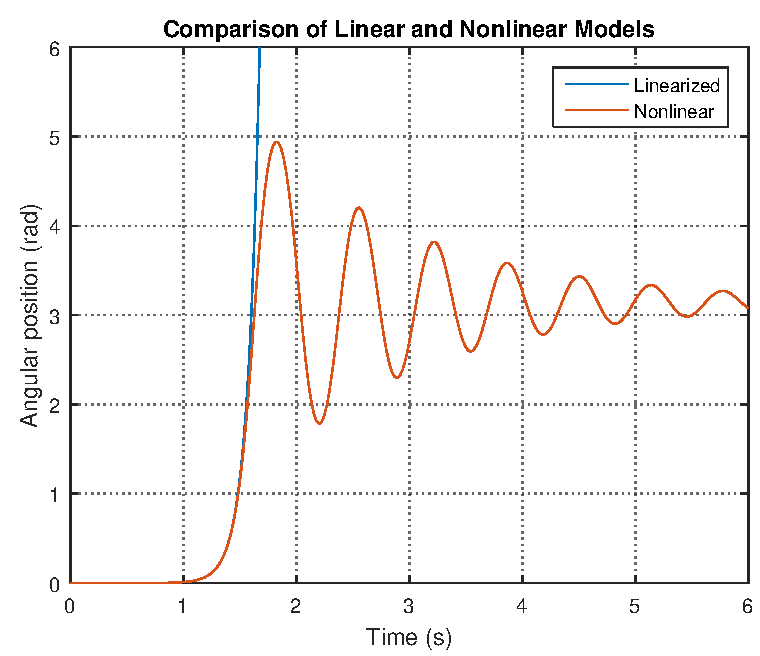
\includegraphics[scale=.5]{figures/LinearizedVSNonlinear}
    	\centering
  		\captionsetup{justification=centering}
  		\captionof{figure}{Simulation of the linearized model compared to the nonlinear model}
  		\label{LinearizedVSNonlinear}
  	\end{figure}
  \end{minipage}
  %	\hspace{0.03\linewidth}
  \begin{minipage}{0.5\linewidth}
  	\begin{figure}[H]%\vspace{4mm}
  		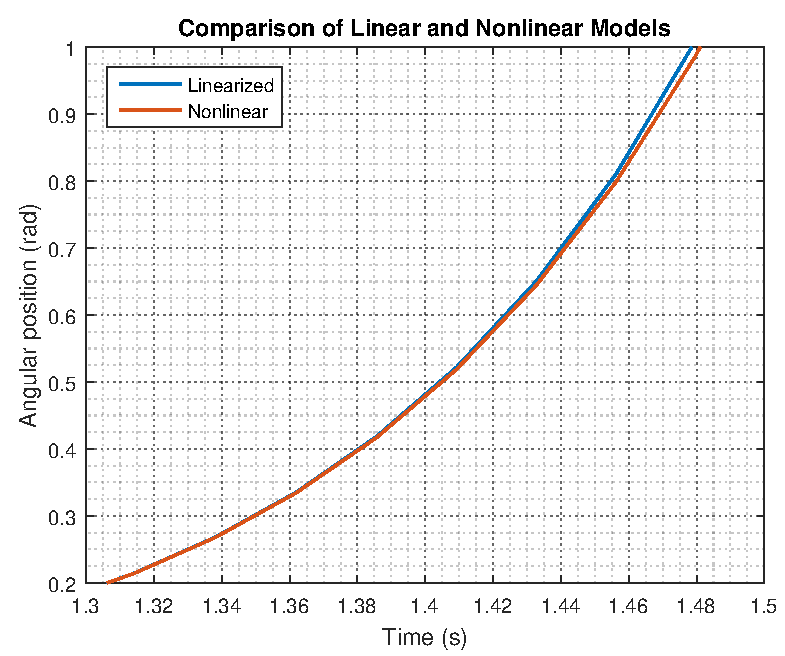
\includegraphics[scale=.5]{figures/LinearizedVSNonlinearZoom}
  		\centering
  		\captionsetup{justification=centering}
  		\captionof{figure}{Zoom of \figref{LinearizedVSNonlinear} from t=1.3s to t=1.5s}
  		\label{LinearizedVSNonlinearZoom}
  	\end{figure}
  \end{minipage}
\end{minipage}

From \figref{LinearizedVSNonlinear} and \figref{LinearizedVSNonlinearZoom}, the linearized model is considered a good approximation of the system's behavior in the operational region of \si{\pm 0,79\ rad}, since the error committed is no more than 0.01 rad at this point.

To further investigate the model, an other test is made, see \appref{fallResponseAppendix}, to determine weather the fall response of the nonlinear model and the real system matches.

\begin{minipage}{\linewidth}
	\begin{minipage}{0.5\linewidth}
		\begin{figure}[H]
			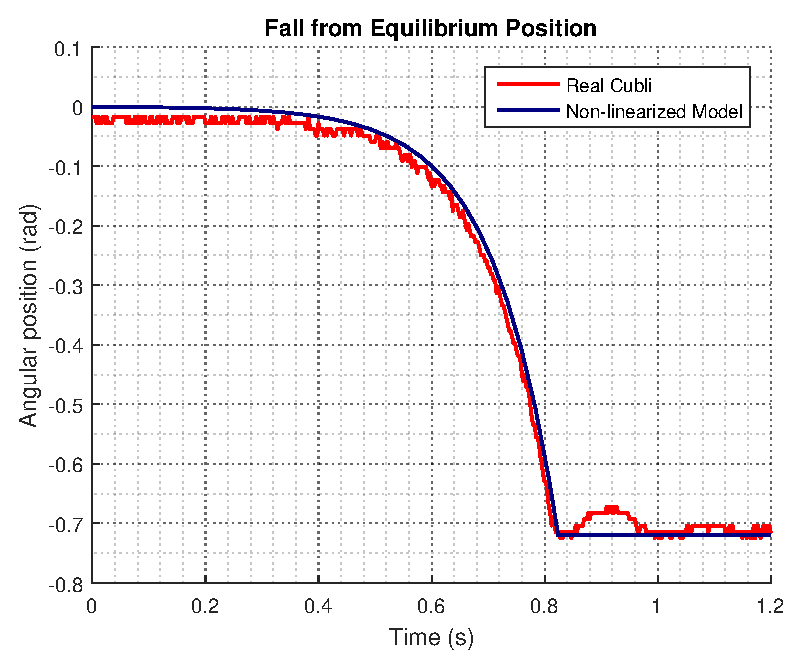
\includegraphics[scale=.48]{figures/FallTestComparison}
			\centering
			\captionsetup{justification=centering}
			\captionof{figure}{Comparison of test and nonlinear model of frame falling from equilibrium position}
			\label{FallTestComparison}
		\end{figure}%\vspace{-5mm}
	\end{minipage}
%	\hspace{0.03\linewidth}
	\begin{minipage}{0.5\linewidth}
		\begin{figure}[H]%\vspace{-4mm}
			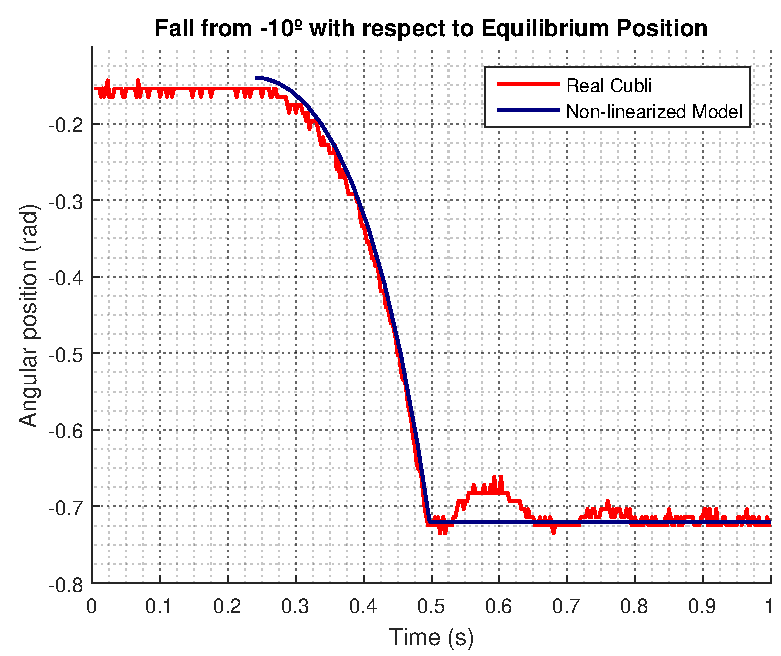
\includegraphics[scale=.48]{figures/FallTestComparison10deg}
			\centering
			\captionsetup{justification=centering}
			\captionof{figure}{Comparison of test and model of frame falling from initial condition \si{-0,174\ rad}}
			\label{FallTestComparison10deg}
		\end{figure}%vspace{-5mm}
	\end{minipage}
\end{minipage}

In \figref{FallTestComparison} the Cubli falls from equilibrium position given a very small impulse. When plotting the two data sets the time of the fall is aligned to see if the characteristics of the simulated fall matches reality.\\
In an attempt to avoid unjustified assumptions the test is repeated from initial condition \si{-0,174\ rad} (\si{-10^\circ}) in both simulation and test, the result is shown in \figref{FallTestComparison10deg}.

%Hence the linearized model is used both for further analysis of the system and for controller design.
